\documentclass[french, 12pt]{article}

%-------------------------------------------------------------------------------
\usepackage[a4paper,top=2cm,bottom=2cm,left=2cm,right=2cm,marginparwidth=1.75cm]{geometry}
\usepackage{amsmath,amsfonts,amssymb,amsthm}
\usepackage[french]{babel}
\usepackage[utf8]{inputenc}
\usepackage[T1]{fontenc}
\usepackage{enumerate}
\usepackage{natbib}
\usepackage{graphicx}
\usepackage{xspace}
\usepackage{color,xcolor}
\usepackage{tikz}
\usepackage{remreset}
\usepackage{url}
\usepackage{boites}
% \usepackage{extsizes} % Permet \documentclass[french, 14pt]{extreport}
% \usepackage[a4paper,top=1cm,bottom=2cm,left=1cm,right=1cm,marginparwidth=.75cm]{geometry}
% \usepackage{minitoc}

\graphicspath{{../Figures/}}

% Environnement
\newtheorem{theorem}{Théorème}
\newtheorem{definition}{Définition}
\newtheorem{lemma}{Lemme}
\newtheorem{proposition}{Proposition}
\newtheorem*{theorem*}{Théorème}
\newtheorem*{definition*}{Définition}
\newtheorem*{proposition*}{Proposition}
\newtheorem*{corollary*}{Corollaire}
\newtheorem*{assumption*}{Hypothèse}
\newtheorem*{algorithm*}{Algorithme}
\newtheorem*{lemma*}{Lemme}
\newtheorem*{remark*}{Remarque}
\newtheorem*{exercise*}{Exercice}
\newtheorem{exercise}{Exercice}
\newcommand{\remark}{\bigskip\noindent\textbf{\textsl{Remarque.}}\xspace}
\newcommand{\remarks}{\bigskip\noindent\textbf{\textsl{Remarques.}}\xspace}
\newcommand{\parSR}[1]{\paragraph*{\textsl{#1}}\xspace}
\renewcommand{\proof}{\bigskip\noindent\underline{\textsl{Démonstration}.}\xspace}
\newcommand{\eproof}{$\blacksquare$}

% Effets, couleurs
\newcommand{\emphase}[1]{\textcolor{red}{#1}}
\newcommand{\demoProp}[1]{\noindent{\textbf{\textsl{Démonstration de la proposition \ref{#1} :}}}}
\newcommand{\itemdot}{\textbullet}

% Moments
\DeclareMathOperator{\Esp}{\mathbb{E}}
\DeclareMathOperator{\diag}{diag}
\DeclareMathOperator{\Cov}{\mathbb{C}ov}
\DeclareMathOperator{\tr}{tr}
\DeclareMathOperator{\Var}{\mathbb{V}}
\let\Pr\relax\DeclareMathOperator{\Pr}{\mathbb{P}}
\renewcommand{\d}{\text{d}}

% R, N, ...
\newcommand{\cst}{\text{cst}}
\newcommand{\Cbb}{\mathbb{C}}
\newcommand{\Ibb}{\mathbb{I}}
\newcommand{\Nbb}{\mathbb{N}}
\newcommand{\Rbb}{\mathbb{R}}
\newcommand{\Zbb}{\mathbb{Z}}

% Indicateurs

% Lois et ensembles
\newcommand{\Acal}{\mathcal{A}}
\newcommand{\Bcal}{\mathcal{B}}
\newcommand{\Ccal}{\mathcal{C}}
\newcommand{\Ecal}{\mathcal{E}}
\newcommand{\Gcal}{\mathcal{G}}
\newcommand{\Ical}{\mathcal{I}}
\newcommand{\Lcal}{\mathcal{L}}
\newcommand{\Mcal}{\mathcal{M}}
\newcommand{\Ncal}{\mathcal{N}}
\newcommand{\Pcal}{\mathcal{P}}
\newcommand{\Rcal}{\mathcal{R}}
\newcommand{\Scal}{\mathcal{S}}
\newcommand{\Ucal}{\mathcal{U}}
\newcommand{\Xcal}{\mathcal{X}}
\newcommand{\Ycal}{\mathcal{Y}}

% Comments
\newcommand{\SR}[2]{\textcolor{gray}{#1}\textcolor{red}{#2}}
\newcommand{\todo}[1]{\textcolor{red}{\`A faire~: {\sl #1}}}
\newcommand{\dessin}[1]{
\begin{center}\framebox{\begin{minipage}{\textwidth}
  \textcolor{purple}{#1}
\end{minipage}}\end{center}
\bigskip
}
\newcommand{\progres}[1]{
\begin{center}\framebox{\begin{minipage}{\textwidth}
  \textcolor{blue}{{\sl #1}}
\end{minipage}}\end{center}
\bigskip
}
\newcommand{\solution}[1]{
\begin{center}\framebox{\begin{minipage}{\textwidth}
  \noindent{\sl Solution :}
  #1
\end{minipage}}\end{center}
\bigskip
}
% \newcommand{\exemple}[1]{
% \begin{center}\framebox{\begin{minipage}{\textwidth}
%   \parSR{Exemple.}
%   #1
% \end{minipage}}\end{center}
% \bigskip
% }
\newcommand{\exemple}[1]{
\begin{breakbox}
  \parSR{Exemple.}
  #1
\end{breakbox}
\bigskip
}

\newcommand{\SRcorrect}[2]{\textcolor{gray}{#1}\textcolor{blue}{#2}}
\newcommand{\SRcomment}[1]{\textcolor{blue}{[{\sl SR: #1}]}}



% Proposition numbering
% \numberwithin{proposition}{section}
\numberwithin{exercise}{section}
\numberwithin{equation}{section}

% Suppression des solutions
\renewcommand{\solution}[1]{}

%-------------------------------------------------------------------------------
%-------------------------------------------------------------------------------
\begin{document}
%-------------------------------------------------------------------------------
%-------------------------------------------------------------------------------

\begin{center}
  \small{\sc \'Ecole normale supérieure de Paris, Licence de Biologie L3, Année 2022-23} \\
  \bigskip
  \large{Ce qu'un biologiste doit savoir en mathématiques} \\
  \bigskip  
  {TD n° 2}
\end{center}

%-------------------------------------------------------------------------------
%-------------------------------------------------------------------------------
\section{Fonctions de plusieurs variables} 
\newcommand{\multivar}{/home/robin/ENSEIGN/Cours/MathBiologie/L3-ENS-Math1/Exercices/MultiVar}
%-------------------------------------------------------------------------------

%-------------------------------------------------------------------------------
\subsection{Normes}
%-------------------------------------------------------------------------------

%-------------------------------------------------------------------------------
\subsubsection{Equivalence des normes}
%-------------------------------------------------------------------------------

Donner des constantes $c_1$ et $c_2$ permettant de comparer les trois normes $\|\cdot\|_1$, $\|\cdot\|_2$ et $\|\cdot\|_\infty$ dans $\Rbb^n$.
\solution{On considère les trois paires de normes.
\begin{description}
  \item[$\|x\|_2$ et $\|x\|_\infty$:] On a vu en cours que
  $$
  \|x\|_\infty \leq \|x\|_2 \leq \sqrt{n} \|x\|_\infty.
%   \qquad \Rightarrow \qquad
%   \frac1{\sqrt{n}} \|x\|_2 \leq \|x\|_\infty \leq \|x\|_2. 
  $$
  \item[$\|x\|_1$ et $\|x\|_\infty$:]  On voit facilement que 
  $$
  \|x\|_\infty \leq \|x\|_1 \leq n \|x\|_\infty.
%   \qquad \Rightarrow \qquad
%   \frac1n \|x\|_1 \leq \|x\|_\infty \leq \|x\|_1.
  $$
  \item[$\|x\|_1$ et $\|x\|_2$:]  On peut déduire une comparaison de $\|x\|_1$ et $\|x\|_2$ en combinant ces résultats
  \begin{align*}
  & \|x\|_1 \leq n \|x\|_\infty \leq n \|x\|_2 \leq n^{3/2} \|x\|_\infty \leq n^{3/2} \|x\|_1 \\
  \Rightarrow \qquad
  & \frac1n \|x\|_1 \leq \|x\|_2 \leq \sqrt{n} \|x\|_1.
%   \Rightarrow \qquad
%   & \frac1{\sqrt{n}} \|x\|_2 \leq \|x\|_1 \leq n \|x\|_2.
  \end{align*}
  On peut cependant affiner les deux constantes :
  \begin{description}
    \item[$\|x\|_2 \leq c_1 \|x\|_1$ :] en définissant, pur $1 \leq i \leq n$, les vecteurs $u_i = x_i e_i$ (où les $e_i$ sont les vecteurs de la base canonique), l'inégalité triangulaire pour la norme $\|\cdot\|_2$ implique que
    $$
    \|x\|_2 \leq \sum_i \|u_i\|_2 = \sum_i |x_i| = \|x\|_1 ;
    $$
    \item[$\|x\|_1 \leq c_2 \|x\|_2$ :] en utilisant le fait que $2ab \leq a^2 + b^2$, il vient
%     la boule unité de la norme $\|\cdot\|_2$ est incluse dans la boule de rayon $\sqrt{n}$ de la norme $\|\cdot\|_1$, il vient que $\|x\|_1 \leq \sqrt{n} \|x\|_2$.
    \begin{align*}
      \|x\|_1^2
      & = \left(\sum_i |x_i|\right)^2
      =  \sum_i |x_i|^2 + \sum_{i < j} 2 |x_i||x_j| \\ 
      & \leq \sum_i |x_i|^2 + \sum_{i < j} (|x_i|^2 + |x_j|^2) 
      = \sum_i |x_i|^2 + \sum_{i \neq j} |x_i|^2 \\
      & = n \sum_i |x_i|^2 = n \|x\|_2^2,
    \end{align*}
    c'est-à-dire : $\|x\|_1 \leq \sqrt{n} \|x\|_2$ ;
  \end{description}
  soit au total
  $$
  \frac1{\sqrt{n}} \|x\|_1 \leq \|x\|_2 \leq \|x\|_1.
  $$
\end{description}
On peut vérifier que les constantes sont optimales en donnant des exemples pour lesquels chacune des égalités est obtenue. Considérons le vecteur $x$ dont toutes les coordonnées sont égales et le vecteur $y$ dont toutes les coordonnées sont nulles, sauf une (par exemple, la première) :
$$
x = a 1_n, \qquad y = b e_1.
$$
On a :
\begin{align*}
  & \text{pour } \|\cdot\|_2 \text{ et } \|\cdot\|_\infty : & 
  \|x\|_2 & = \sqrt{n} \|x\|_\infty, & 
  \|y\|_2 & = \|y\|_\infty; \\
  & \text{pour } \|\cdot\|_1 \text{ et } \|\cdot\|_\infty : & 
  \|x\|_1 & = n \|x\|_\infty, & 
  \|y\|_1 & = \|y\|_\infty; \\
  & \text{pour } \|\cdot\|_1 \text{ et } \|\cdot\|_2 : & 
  \|y\|_2 & = \|y\|_1, &
  \|x\|_1 & = \sqrt{n} \|x\|_2.
\end{align*}
}



%-------------------------------------------------------------------------------
\subsubsection{Norme fondée sur une matrice définie positive}
%-------------------------------------------------------------------------------

  Soit $A$ une matrice de $\Mcal_n$ symétrique définie positive (strictement): $A \succ 0$. Montrer que $\|\cdot\|_A$ définie par $\|x\|_A = (x^\top A x)^{1/2}$ est une norme pour $\Rbb^n$.
\solution{On vérifie les 3 conditions définissant une norme.
  \begin{enumerate}
   \item Par définition des matrices définies positives, on a bien pour tout $x \in \Rbb^n$, $x^\top A x \geq 0$  et $\{x^\top A x = 0\} \Leftrightarrow \{x = 0\}$.
   \item On a également $\|\lambda x\|_A = ((\lambda x)^\top A (\lambda x))^{1/2} = (\lambda^2 x^\top A x)^{1/2} = |\lambda| \|x\|_A$ ;
   \item Puisque $A$ est symétrique, on a
   $$
   \|x + y\|^2_A 
   = \|x\|^2_A + \| y\|^2_A + 2 x^\top A y
   $$
   et on peut la décomposer sous la forme $A = P \Lambda P^\top$ où $P$ et $P^\top$ sont orthonormales. Posons $u = \Lambda^{1/2} P^\top x$ et $v = \Lambda^{1/2} P^\top y$ qui vérifient
   \begin{align*}
   \|u\|_2 & = \sqrt{x^\top P \Lambda^{1/2} \Lambda^{1/2} P^\top x} = \|x\|_A, & 
   \|v\|_2 & = \|y\|_A, \\
   x^\top A y & = u^\top v.
   \end{align*}
   Par Cauchy-Schwarz, on a alors
   \begin{align*}
    \|x + y\|^2_A 
    & = \|u\|^2_2 + \|v\|^2_2 + 2 u^\top v \leq \|u\|^2_2 + \|v\|^2_2 + 2 |u^\top v| \\
    & \leq \|u\|^2_2 + \|v\|^2_2 + 2 \|u\|_2 \|v\|_2 = (\|u\|_2 + \|v\|_2)^2 \\
    & = (\|x\|_A + \|y\|_A)^2.    
   \end{align*}
  \end{enumerate}
}



%-------------------------------------------------------------------------------
\subsection{Calcul différentiel}
%-------------------------------------------------------------------------------

%-------------------------------------------------------------------------------
\subsubsection{Courbe paramétrée par le temps}
%-------------------------------------------------------------------------------

On considère une fonction 
$$
\begin{array}{rrcl}
  F : & \Rbb & \mapsto & \Rbb^2 \\
  & (x, y) & \to & F(t) 
  = \left(\begin{array}{c} x(t) \\ y(t) \end{array}\right)
  = \left(\begin{array}{c} t - t^3 \\ t^2 - t^4 \end{array}\right)
\end{array}.
$$
\'Etudier cette fonction et tracer son graphe $F(\Rbb)$.
\solution{
  \begin{description}
    \item[Symétrie :] on remarque que
    $$
    x(-t) = -x(t), \qquad y(-t) = y(t)
    $$
    On se contente d'étudier la courbre pour $t \in \Rbb^+$.
    \item[Limites :] on a 
    $$
    \lim_{t \to \infty} x(t) = \lim_{t \to \infty} y(t) = - \infty.
    $$
    \item[En $t = 0$:] on a $x(0) = y(0) = 0$. 
    \item[Coordonnées nulles :] on a
    $$
    x(t) = 0 \quad \Leftrightarrow \quad t \in \{0, 1\}, \qquad
    y(t) = 0 \quad \Leftrightarrow \quad t \in \{0, 1\} ,
    $$
    les coordonnées s'annulent donc simultanément 2 fois en $t = 0$ et $1$.
    \item[Dérivées :] le signe des dérivées est donné par
    \begin{align*}
      \dot x(t) & \geq 0 & & \Leftrightarrow & 1 - 3t^2 & \geq 0 & & \Leftrightarrow & t & \leq 1/\sqrt{3}, \\
      \dot y(t) & \geq 0 & & \Leftrightarrow & 2t(1 - t^2) & \geq 0 & & \Leftrightarrow & t & \leq 1/\sqrt{2}.
    \end{align*}
    \item[Tableau de variation :] on a donc 
%     en complétant la partie $t \in \Rbb^-$ par symétrie, 
    $$
%     \begin{array}{c|cccccccccccccccccc}
%       t & -\infty & & -1 & & -\frac1{\sqrt{2}} & & -\frac1{\sqrt{3}} & & 0 & & \frac1{\sqrt{3}} & & \frac1{\sqrt{2}} & & 1 & & +\infty \\
%       \hline
%       \dot x & & - & & - & & - & 0 & + & & + & 0 & - & & - & & - & \\
%       x & + \infty & \searrow & 0 & \searrow & \frac{-1}{2\sqrt{2}} & \searrow & \frac{-2}{3\sqrt{3}} & \nearrow & 0 & \nearrow & \frac{2}{3\sqrt{3}} & \searrow & \frac{1}{2\sqrt{2}} & \searrow & 0 & \searrow & - \infty \\
%       \hline
%       \dot y & & + & & + & 0 & - & & - & 0 & + & & + & 0 & - & & - & \\
%       y & - \infty & \nearrow & 0 & \nearrow & \frac14 & \searrow & \frac29 & \searrow & 0 & \nearrow & \frac29 & \nearrow & \frac14 & \searrow & 0 & \searrow & - \infty \\
%     \end{array}
    \begin{array}{c|cccccccccccccccccc}
      t & 0 & & 1/{\sqrt{3}} & & 1/{\sqrt{2}} & & 1 & & +\infty \\
      \hline
      \dot x & & + & 0 & - & & - & & - & \\
      x & 0 & \nearrow & 2/{3\sqrt{3}} & \searrow & 1/{2\sqrt{2}} & \searrow & 0 & \searrow & - \infty \\
      \hline
      \dot y & 0 & + & & + & 0 & - & & - & \\
      y & 0 & \nearrow & 2/9 & \nearrow & 1/4 & \searrow & 0 & \searrow & - \infty \\
    \end{array}
    $$
    
    \item[Graphe $F(\Rbb)$ :] on a ainsi
    $$
    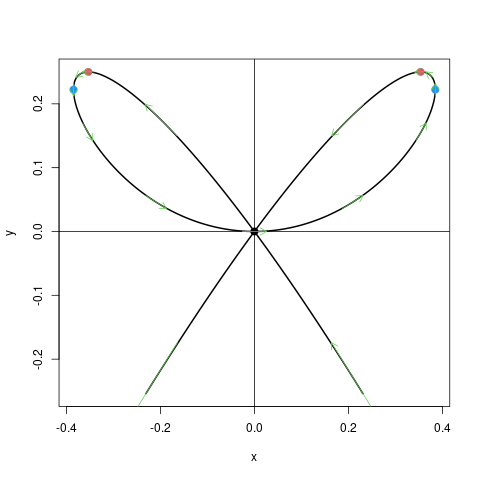
\includegraphics[width=.5\textwidth]{CourbeParametreeDim2}
    $$
  \end{description}

}


%-------------------------------------------------------------------------------
\subsubsection{Jacobienne de $F \circ F$}
%-------------------------------------------------------------------------------

On considère une fonction 
$$
\begin{array}{rrcl}
  F : & [0, 1] \times [0, 1] & \mapsto & [0, 1] \times [0, 1] \\
  & (x, y) & \to & F(x, y) = (f_1(x, y), f_2(x, y))
\end{array}
$$
\begin{enumerate}
  \item \'Ecrire la matrice jacobienne $J(x, y)$ de la fonction $F$ en tout $(x, y) \in [0, 1] \times [0, 1]$.
  \solution{Par définition, on a
  $$
  J_{(x, y)} F = \left[\begin{array}{cc}
                        f'_{1x}(x, y) & f'_{1y}(x, y) \\
                        f'_{2x}(x, y) & f'_{2y}(x, y)
                       \end{array}\right] 
                       \qquad \text{où} \quad 
  f'_{1x}(x, y) = \left.\frac{\partial f_1}{\partial x}\right|_{(x, y)}.
  $$
  }
  \item \'Ecrire l'application linéaire tangente de $F \circ F$ en tout point $(x, y)$.
  \solution{Par définition, on a
  \begin{align*}
    J_{(x, y)} F \circ F 
    & = J_{(x, y)} F \cdot J_{F(x, y)} F \\
    & = \left[\begin{array}{cc}
          f'_{1x}(x, y) & f'_{1y}(x, y) \\
          f'_{2x}(x, y) & f'_{2y}(x, y)
        \end{array}\right]
        \left[\begin{array}{cc}
          f'_{1x}(F(x, y)) & f'_{1y}(F(x, y)) \\
          f'_{2x}(F(x, y)) & f'_{2y}(F(x, y))
        \end{array}\right].
  \end{align*}
  L'application linéaire tangente au point $(x^*, y^*)$ est donc
  \begin{align*}
  L_{(x^*, y^*)}(x, y) 
  & = F(F(x^*, y^*)) \\
  & \qquad + (f'_{1x}(x^*, y^*) f'_{1x}(F(x^*, y^*)) + f'_{1y}(x^*, y^*) f'_{2x}(F(x^*, y^*))) x \\
  & \qquad +(f'_{2x}(x^*, y^*) f'_{1y}(F(x^*, y^*)) + f'_{2y}(x^*, y^*) f'_{2y}(F(x^*, y^*))) y 
  \end{align*}}
  \item On suppose que $F(1, 1) = (1, 1)$. Donner la matrice jacobienne $J_n(1, 1)$ de la fonction $F$ itérée $n$ fois avec elle-même, en $(x, y) = (1, 1)$.
  \solution{On a alors $J_{F(1, 1)}F = J_{(1, 1)}F$, soit
  $$
  J_2(1, 1)
  = J_{(1, 1)} F \circ F 
  = J_{(1, 1)} F \cdot J_{F(1, 1)} F 
  = \left(J_{(1, 1)} F\right)^2.
  $$
  Par récurrence, puisque
  $$
  J_{(x, y)} F^n 
  = J_{(x, y)} (F^{n-1} \circ F)
  = J_{(x, y)} F \cdot J_{F(x, y)} F^{n-1},
  $$
  il vient
  $$
  J_n(1, 1) = \left(J_{(1, 1)} F\right)^n.
  $$
  }
\end{enumerate}



%-------------------------------------------------------------------------------
%-------------------------------------------------------------------------------
\section{\'Equations différentielles et systèmes dynamiques} 
\newcommand{\equadiff}{/home/robin/ENSEIGN/Cours/MathBiologie/L3-ENS-Math1/Exercices/EquaDiff}
%-------------------------------------------------------------------------------

%-------------------------------------------------------------------------------
\subsection{Systèmes dynamiques en dimension 1}
%-------------------------------------------------------------------------------

%-------------------------------------------------------------------------------
\subsubsection{Modèle cubique}
%-------------------------------------------------------------------------------

% [Exercice 2, TD2, L2 Bio SU]

\exemple{
  On considère le système
  $$
  \dot y = - y^3 + 7 y^2 - 14 y + 8.
  $$
  Ses points stationnaires sont les racines du polynôme $P(y) = - y^3 + 7 y^2 - 14 y + 8$, donc $y_1 = 1$ fait partie, donc
  $$
  P(y) = (y-1) (-y^2 + 6y + 8),
  $$
  et les deux racines de $-y^2 + 6y + 8$ sont $2$ et $4$. Les points stationnaires du système sont donc 
  $$
  y_1 = 1, \qquad y_2 = 2, \qquad y_3 = 4.
  $$
  Leur stabilité est donné par la dérivée de $P$:
  $$
  P'(y) = -3y^2 + 14 y - 14,
  $$
  soit
  $$
  P'(y_1) = -3, \qquad P'(y_2) = 2, \qquad P'(y_3) = -6.
  $$
  $y_1$ et $y_3$ sont donc des équilibres stables, et $y_2$ un équilibre instable.
  $$
  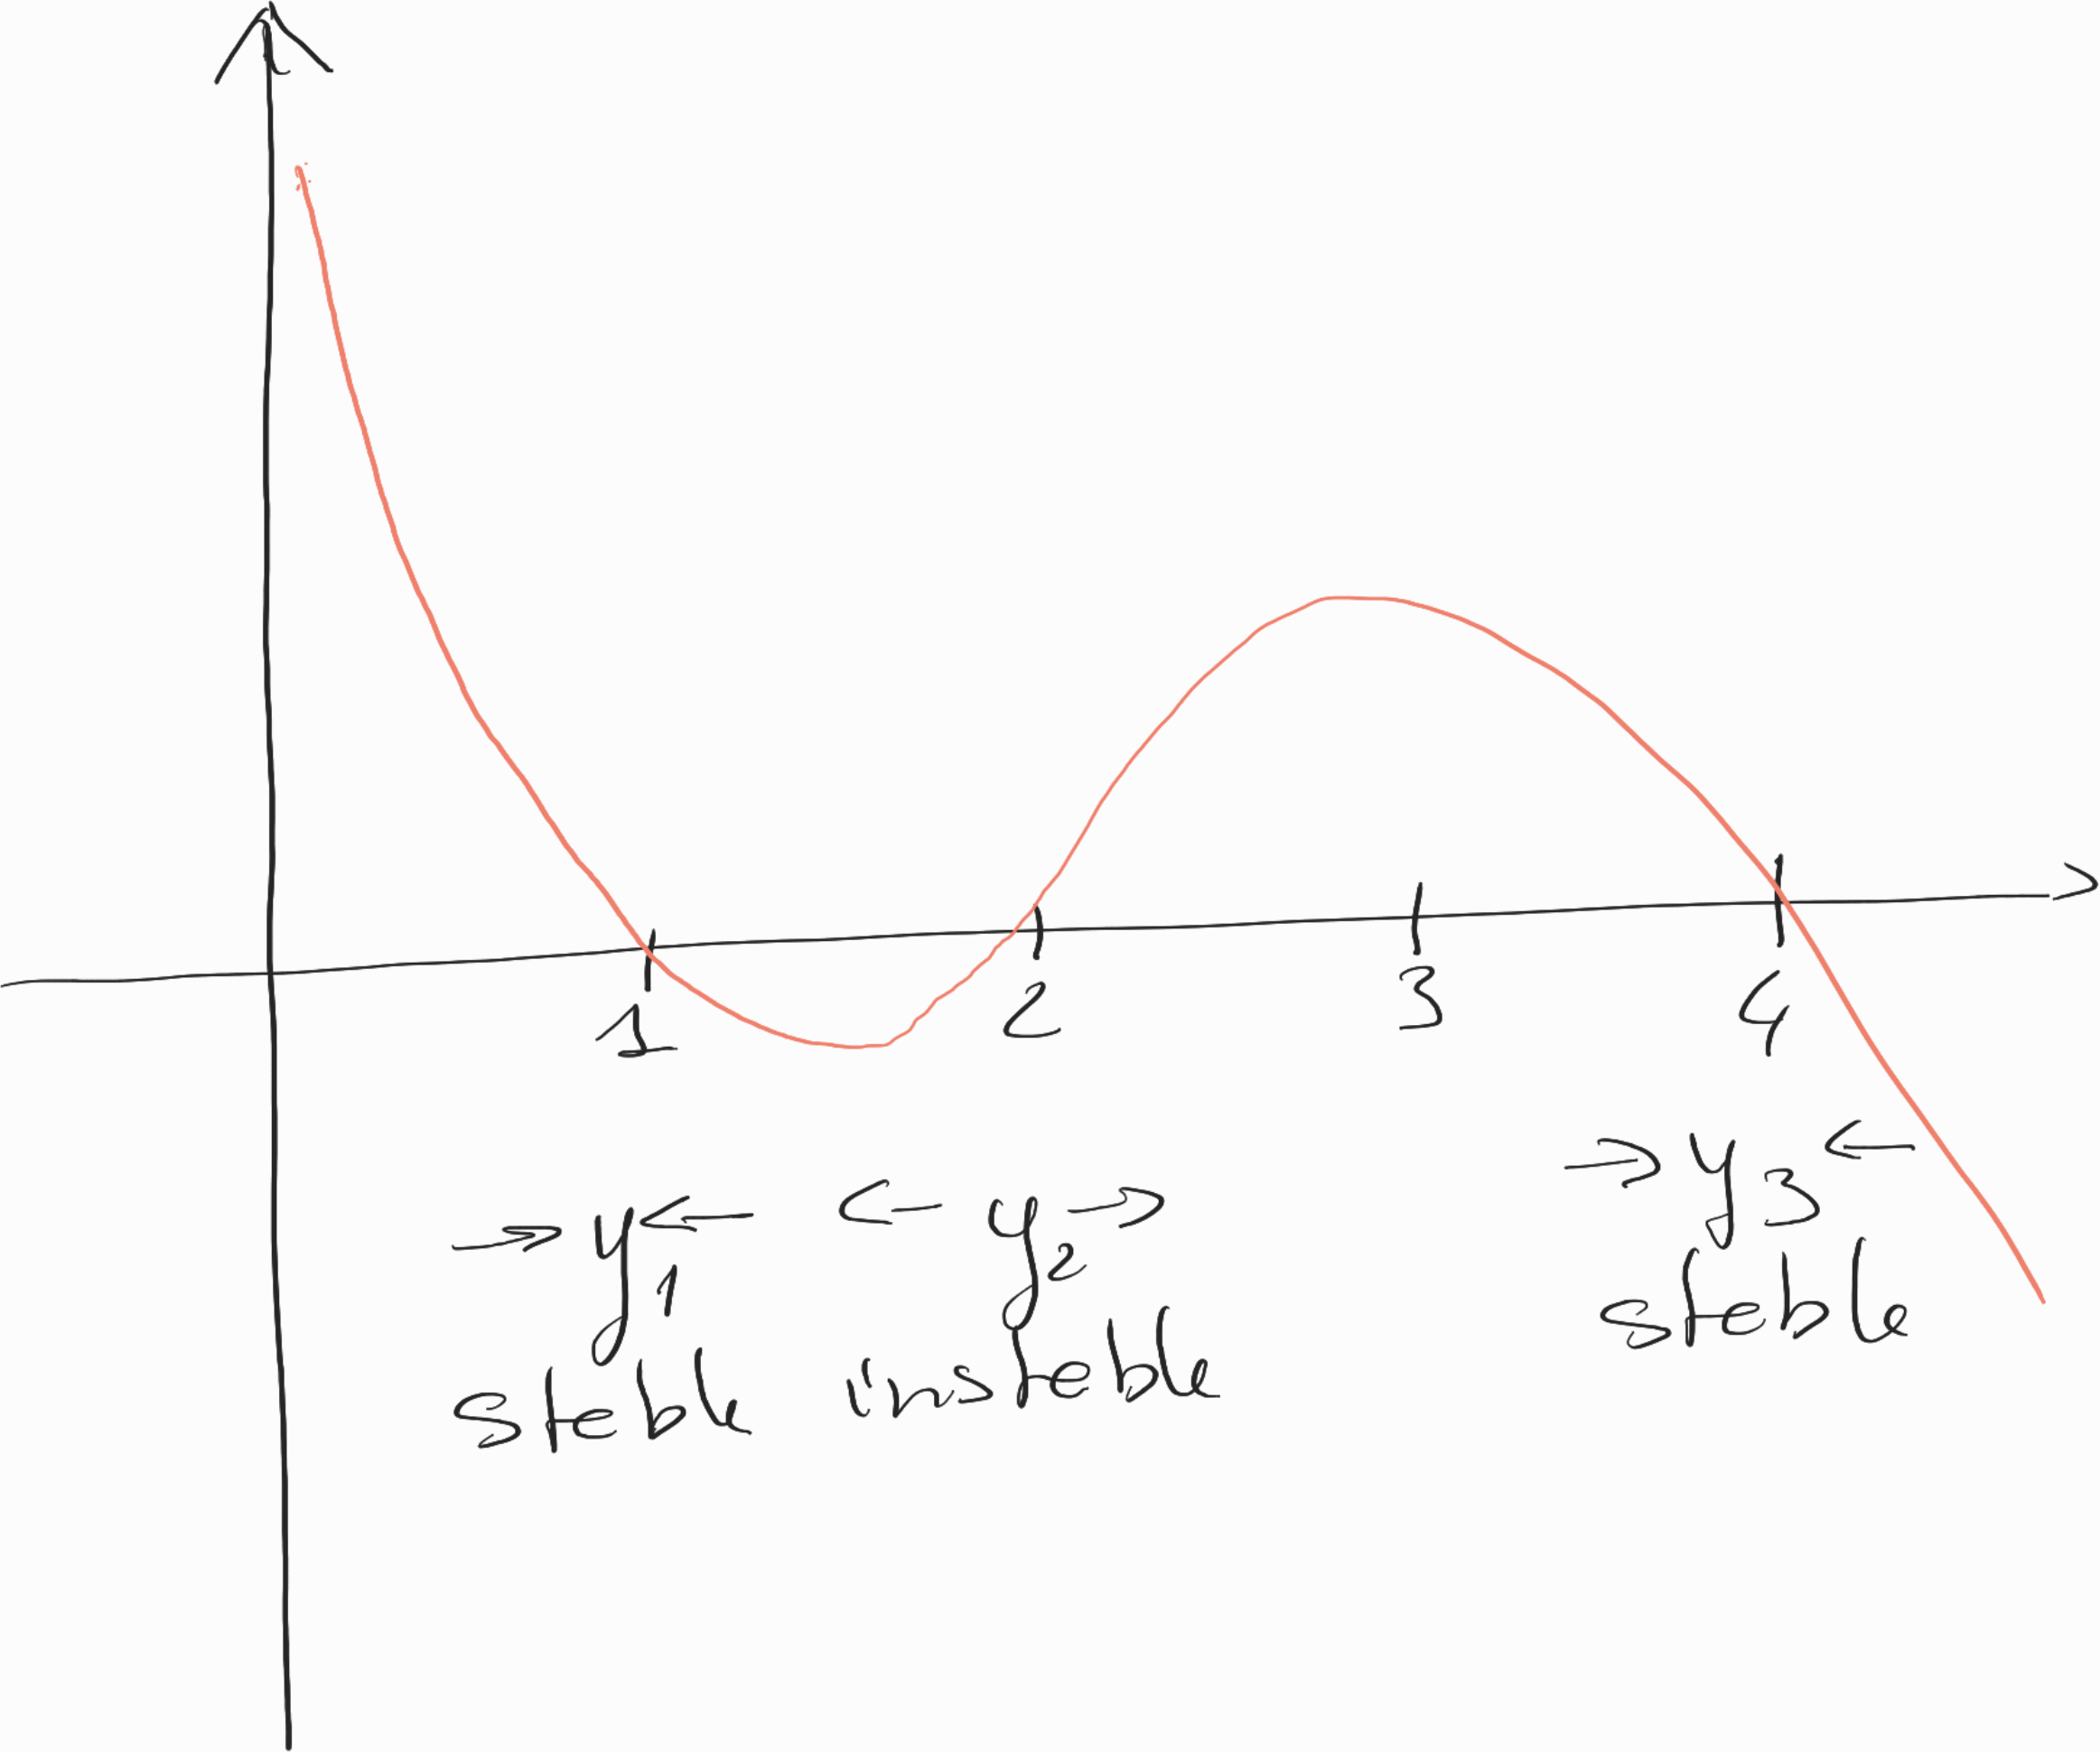
\includegraphics[width=.5\textwidth]{TD-SUbioL3-TD2Exo2}
  $$
}




%-------------------------------------------------------------------------------
\subsection{Systèmes dynamiques en dimension 2}
%-------------------------------------------------------------------------------

%-------------------------------------------------------------------------------
\subsubsection{Système dynamique quadratique} \label{SystDyn-Quadratique}
%-------------------------------------------------------------------------------

On considère le système dynamique d’activation réciproque avec compétition intraspécifique suivant 
$$
%   \SR{
%   \left\{\begin{array}{rcl}
%          \dot x & = & r y - cx^2 \\ 
%          \dot y & = & r x - cy^2 
%          \end{array}\right.
%   }{
\left\{\begin{array}{rcl}
        \dot x & = & a y - x^2 \\ 
        \dot y & = & a x - y^2 
        \end{array}\right.
%   }
$$
%   où $r$ et $c$ sont deux constantes strictement positives.
où $a$ est une constante strictement positive.
\begin{enumerate}
  \item Déterminer les équilibres de ce modèle.
  \solution{$(x=0, y=0)$ est un point d'équilibre trivial. L'autre point d'équilibre s'obtient en résolvant
  $$
  \left\{\begin{array}{rcl}
          a y & = & x^2 \\
          a x & = & y^2
        \end{array}\right.
  \quad \Leftrightarrow \quad
  \left\{\begin{array}{rcl}
          y & = & x^2 / a \\
          a x & = & x^4 / a^2
        \end{array}\right.
  \quad \Leftrightarrow \quad
  \left\{\begin{array}{rcl}
          y & = & x^2 / a \\
          a^3 & = & x^3
        \end{array}\right.
  \quad \Leftrightarrow \quad
  x^* = y^* = a.
  $$}
  \item Donner la nature de chacun de ces deux équilibres.
  \solution{En notant
  $$
  F(x, y) = \left[\begin{array}{rcl} 
                    F_1(x, y) & = & ay - x^2 \\
                    F_2(x, y) & = & ax - y^2
                  \end{array}\right],
  $$
  on a
  $$
  J_{(x, y)} F = \left[\begin{array}{cc}-2x & a \\ a & -2y\end{array}\right].
  $$
  \begin{description}
    \item[Point $(0, 0)$:] on a
    $$
    J_{(0, 0)} F = \left[\begin{array}{cc}0 & a \\ a & 0\end{array}\right]
    \quad \Rightarrow \quad
    P(\lambda) = \lambda^2 - a^2
    $$
    qui s'annule pour $\lambda = \pm a$. Des vecteurs associés à $a$ et $-a$ sont, respectivement $[1 \; 1]^\top$ et $[-1 \; 1]^\top$. \\
    $(0, 0)$ est un équilibre instable dans la direction de la première bissectrice et stable dans celle de la seconde.
    \item[Point $(a, a)$:] on a
    $$
    J_{(0, 0)} F = \left[\begin{array}{cc}-2a & a \\ a & -2a\end{array}\right]
    \quad \Rightarrow \quad
    P(\lambda) = \lambda^2 - a^2
    \quad \Rightarrow \quad
    P(\lambda) = \lambda^2 - 4 a \lambda + 3 a^2
    $$
    qui s'annule pour $\lambda = -a$ et $\lambda = -3a $. \\
    $(a, a)$ est donc un équilibre stable.
  \end{description}
  }
  \item Que se passe-t-il si $x(0) = y(0) > 0$ ? Représenter l’allure des trajectoires dans le plan de phase. 
  \solution{
  On peut remarquer que 
  $$
  \dot x \geq 0 \quad \Leftrightarrow \quad y \geq x^2/a, \qquad \qquad
  \dot y \geq 0 \quad \Leftrightarrow \quad y \leq \sqrt{a x}.
  $$
  $$
  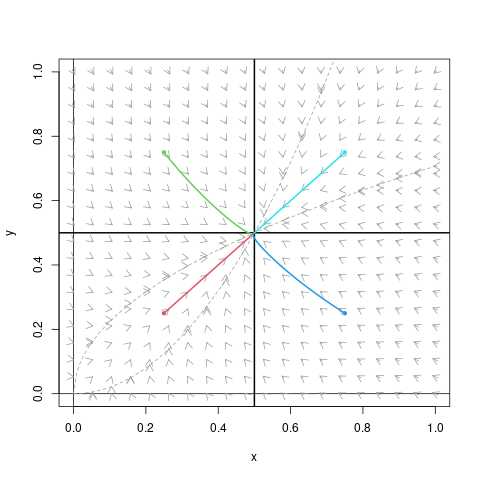
\includegraphics[width=.45\textwidth, trim=0 10 20 20, clip=]{ActivationReciproque}
  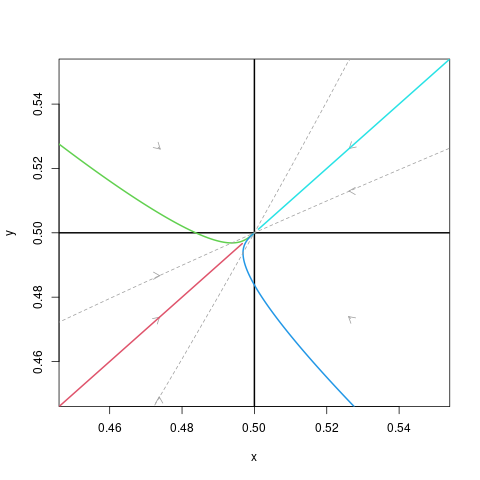
\includegraphics[width=.45\textwidth, trim=0 10 20 20, clip=]{ActivationReciproque-zoom}
  $$
  Toutes les trajectoires convergent vers $(a, a)$.
  \begin{description}
    \item[$(x_0 < a, y_0 < a)$:] la trajectoire converge directement vers $(a, a)$.
    \item[$(x_0 < a, y_0 > a)$:] la trajectoire franchit l'axe $y = a$ avant de revenir en $(a, a)$.
    \item[$(x_0 > a, y_0 > a)$:] la trajectoire converge directement vers $(a, a)$.
    \item[$(x_0 > a, y_0 < a)$:] la trajectoire franchit l'axe $x = a$ avant de revenir en $(a, a)$.
  \end{description}
  }
\end{enumerate}



%-------------------------------------------------------------------------------
\subsection{Dynamique des populations}
%-------------------------------------------------------------------------------

%-------------------------------------------------------------------------------
\subsubsection{Dynamique de population à trois classes : mâles, femelles et couples}
%-------------------------------------------------------------------------------

On considère une population sexuée panmictique, au sein de laquelle on désigne
respectivement par $x(t)$, $y(t)$ et $z(t)$ les densités au temps $t$ de femelles flottantes, de mâles flottants, et de couples. On suppose que la dynamique de la population respecte le système dynamique suivant
\begin{equation} \label{eq:Dyn3Pop}
  \left\{\begin{array}{rcl}
          \dot x(t) & = & - \alpha x y + r z, \\
          \dot y(t) & = & - \alpha x y + r z, \\
          \dot z(t) & = & + \alpha x y - c z^2,
          \end{array} \right.
\end{equation}
où les coefficients $\alpha$, $r$ et $c$ sont strictement positifs.
\begin{enumerate}
  \item Interpréter ces équations et la signification de chacun des coefficients $\alpha$, $r$ et $c$.
  \solution{Les mâles et femelles flottant(e)s s'apparient pour former des couples : 
  \begin{itemize}
    \item $\alpha$ est le taux de formation des couples, 
    \item $r$ est le taux de natalités de mâles et des femelles (supposés égaux),
    \item $c$ est le taux de mortalité des couples.
  \end{itemize}
  }
  \item En notant $S = x(0) - y(0)$, montrer que $x(t) - y(t) = S$ pour tout temps $t$. En
  déduire les fonctions $y$ et $z$ satisfont le système 
  \begin{equation} \label{eq:Dyn3Pop2}
    \left\{\begin{array}{rcl}
            \dot y(t) & = & - \alpha (y^2 + Sy) + r z, \\
            \dot z(t) & = & + \alpha (y^2 + Sy) - c z^2.
            \end{array} \right.
  \end{equation}
  Dans la suite on supposera que $S > 0$.
  \solution{On remarque que
  $$
  \dot x(t) - \dot y(t) = 0,
  $$
  ce qui implique que la différence $x(t) - y(t)$ reste constante au cours du temps et égale à $x(0) - y(0) = S$. \\
  On peut donc remplacer $x(t) = y(t) + S$ dans le système \eqref{eq:Dyn3Pop} pour obtenir le système \eqref{eq:Dyn3Pop2}.}
  \item Déterminer les points d'équilibre du système \eqref{eq:Dyn3Pop2}.
  \solution{
  \begin{itemize}
    \item $(y^* = 0, z^* = 0)$ est un équilibre (trivial).
    \item $(y = -S, z^* = 0)$ n'est pas un équilibre intéressant du point de vue du modèle car on s'intéresse aux effectifs positifs ou nuls. 
    \item Si on suppose $({y^*}^2 + Sy^*) \neq 0$, il vient
    $$
    \alpha({y^*}^2 + Sy^*) = rz^* = c{z^*}^2 
    \qquad \Rightarrow \qquad 
    z^* = r / c
    $$
    et $y^*$ doit vérifier
    $$
    {y^*}^2 + Sy^* - \frac{r^2}{\alpha c} = 0,
    $$
    dont le discriminant est 
    $$
    \Delta =  S^2 + \frac{4 r^2}{\alpha c} > S^2,
    $$
    et dont la seule solution positive est
    $$
    y^* = \frac{\sqrt{\Delta} - S}2.
    $$
    Le second équilibre intéressant est donc $(y^* = (\sqrt{\Delta} - S)/2, z^* = r/c)$. \\
    $(y^* = (-\sqrt{\Delta} - S)/2, z^* = r/c)$ est bien un point d'équilibre, mais sans intérêt du point de vue du modèle.
  \end{itemize}
  }
  \item \'Ecrire la matrice jacobienne du système \eqref{eq:Dyn3Pop2} et étudier la nature du ou des équilibres non triviaux.
  \solution{La jacobienne vaut
  $$
  J = \left[\begin{array}{rr}
              -2 \alpha y - \alpha S & r \\ 2 \alpha y + \alpha S & -2 c z
            \end{array}\right]
  $$
  \begin{description}
    \item[En $(0, 0)$ :] on a 
    $$
    J_{(0, 0)} = \left[\begin{array}{rr}
                - \alpha S & r \\ \alpha S & 0
              \end{array}\right]
    \qquad \Rightarrow \qquad
    P(\lambda) = \lambda^2 + \alpha S \lambda - r \alpha S
    $$
    où
    $$
    \Delta_0 = \alpha^2 S^2 (1 - 4 r / (\alpha S)).
    $$
    \begin{itemize}
      \item Si $\Delta_0 \geq 0$, les deux valeurs propres
      $$
      \lambda = \frac{\alpha S}2 \left(-1 \pm \sqrt{1 - 4r/(\alpha S)}\right)
      $$
      sont négatives (car $\sqrt{1 - 4r/(\alpha S)} < 1$) et $(0, 0)$ est un équilibre stable. 
      \item Si $\Delta_0 < 0$, la partie réelle ($-\alpha S/2$) des deux valeurs propres est négative et l'équilibre est également stable.
    \end{itemize}
    \item[En $(y^* = \sqrt{\Delta} - S)/2, z^* = r/c)$ :] on a 
    $$
    J_{(y^*, z^*)} = \left[\begin{array}{rr}
                - \alpha \delta & r \\ \alpha \delta & -2 r
              \end{array}\right]
    \qquad \Rightarrow \qquad
    P(\lambda) = \lambda^2 + (\alpha \delta + 2r) \lambda - r \alpha \delta,
    $$
    en notant $\delta = 2(\sqrt{\Delta} - S) + S = 2\sqrt{\Delta} - S > 0$. On a cette fois
    $$
    \Delta^* 
    = \frac12 \left((\alpha \delta + 2r)^2 - 4 r \alpha \delta\right)
    = \frac12 (\alpha \delta - 2r)^2 \geq 0,
    $$
    soit
    $$
    \lambda = \frac12 \left(-(\alpha \delta + 2r) \pm \sqrt{\Delta^* }\right) \leq 0
    $$
    car, les coefficients $\alpha$, $r$ et $c$ étant tous positifs,
    $$
    \frac12 (\alpha \delta - 2r)^2 < (\alpha \delta + 2r)^2.
    $$
    $(y^* = \sqrt{\Delta} - S)/2, z^* = r/c)$ est donc un équilibre stable.
    
  \end{description}
  $$
  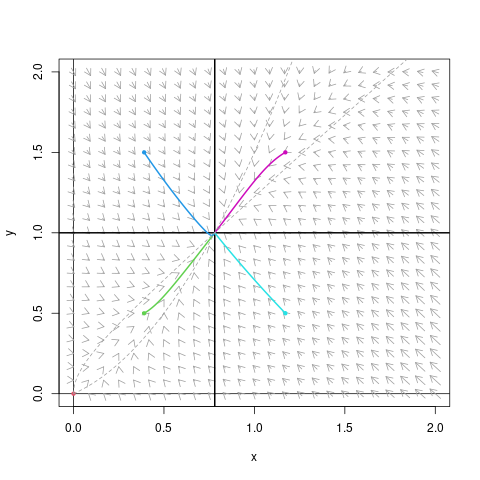
\includegraphics[width=.5\textwidth]{DynPopMaleFemelleCouple.png}
  $$
  }
\end{enumerate}



%-------------------------------------------------------------------------------
%-------------------------------------------------------------------------------
\end{document}
%-------------------------------------------------------------------------------
%-------------------------------------------------------------------------------


